\documentclass{article}

% Numeric, range-compressed citations. Author-year is natbib's default here and
% renders \cite inline as "evict idle caches Kwon et al. [2023]", which reads as
% a sentence fragment; it also costs several lines in a 4-page budget, since a
% four-work citation group becomes four full author strings instead of "[10-13]".
\PassOptionsToPackage{numbers,compress}{natbib}

% Workshop track, single-blind. The ML for Systems CFP says review is non-blind
% ("Submissions do not have to be anonymized"), and sglblindworkshop is the option
% that renders the real author block.
%
% Deliberately WITHOUT `final`. The official template reserves that for after
% acceptance ("the authors should add 'final' behind the track to compile a
% camera-ready version"). Submission mode is correct here: it keeps the reviewer
% line numbers and the "Submitted to ... Do not distribute" banner, which is what
% a paper under review should carry.
\usepackage[sglblindworkshop]{neurips_2026}
\workshoptitle{Machine Learning for Systems}

\usepackage[utf8]{inputenc}
\usepackage[T1]{fontenc}
% [draft] is required in submission mode. The style file loads `lineno` when
% `final` is absent, and a hyperlink straddling a page break under `lineno`
% aborts the build with "This can't happen (pdfvlistout)". [draft] keeps every
% hyperref command working but emits no link objects, which sidesteps it; URLs
% still render as text. Drop [draft] together with the switch to `final` at
% camera-ready, when `lineno` goes away.
\usepackage[draft]{hyperref}
\usepackage{url}
\usepackage{booktabs}
\usepackage{amsmath,amsfonts}
\usepackage{nicefrac}
\usepackage{microtype}
\usepackage{xcolor}
\usepackage{graphicx}

\title{Hit Rate Is Not Value: When Cache Metrics Mislead\\in Tiered LLM KV-Cache Persistence\thanks{System, committed run records, and the scripts regenerating every number, figure, and table here: \url{https://github.com/aditya-lawankar/kv-cache-tier-persistence}}}

\author{%
  Aditya Lawankar \\
  \texttt{lawankaraditya@gmail.com} \\
}

\begin{document}

\maketitle

\begin{abstract}
We set out to beat LRU at evicting persisted LLM KV caches with a learned policy, and failed: across three synthetic workloads, two served architectures, and a replay of the Azure LLM inference trace, LRU wins cache hit rate every time. The interesting result is what that verdict conceals. Measured in GPU time actually saved, the same LRU delivers the \emph{least} value of any policy we test on enterprise traffic, where a value-density policy conceding 21 hit-rate points saves $1.99\times$ as much compute, and still $1.15\times$ once we correct a provisioning error the same analysis exposes. Hit rate assumes every hit is worth the same; KV caching violates that twice, since a hit below the break-even context length $N^{*}$ is worth nothing and above it savings grow superlinearly. Both effects are closed-form in $N^{*}$, and the largest lever they expose is provisioning, not policy: deleting a tier that cannot repay its restore is worth $3.6\times$ at identical capacity. A ground-truth ablation isolates the failure: two clairvoyant policies that both cache perfectly, 100.0\% against 100.0\%, still deliver significantly different value.
\end{abstract}

\section{Introduction}

Serving a large language model proceeds in two phases: \emph{prefill} processes the prompt in parallel and populates the KV cache, and \emph{decode} generates one token at a time against it. Prefill costs $O(N^2)$ attention FLOPs while the cache grows only linearly in $N$, so the cache makes multi-turn boundaries cheap. VRAM has no room for idle sessions, though: an 80\,GB A100 fits only ${\sim}30$ full-context Llama-2-7B sessions after weights, against thousands of users whose think time spans seconds to days. Serving engines therefore evict idle caches~\cite{kwon2023pagedattention}, and a returning user re-prefills everything. Tiered persistence demotes those caches down a hierarchy (VRAM $\to$ NVMe $\to$ object storage), paying $O(N)$ bytes moved instead of $O(N^2)$ FLOPs recomputed~\cite{gao2024cachedattention,qin2025mooncake,zhong2024lmcache}. That relocates the eviction problem rather than eliminating it, since every tier is finite.

That decision looks like fertile ground for learning. Sessions differ by orders of magnitude in size, their recompute cost grows quadratically where their footprint grows linearly, and whether a user returns looks predictable from history. LRU sees none of this, so we hypothesized that a learned policy estimating resumption probability would beat it on hit rate. \emph{The data falsified this hypothesis}, and diagnosing why became the contribution: LRU wins hit rate on every constrained workload, and no feature engineering closed the gap. But the metric was the problem: measured by GPU time saved, that same LRU delivers the \emph{least} value of any policy on enterprise traffic, and policies losing to it by 11--21 hit-rate points save up to twice as much. Hit rate assumes every hit is worth the same, and KV caching breaks that twice: a hit below the break-even length $N^{*}$ is worth \emph{nothing}, and above it savings grow superlinearly (\S\ref{sec:mech}).

\textbf{Related work.} Systems that persist, disaggregate, or offload KV state across a hierarchy~\cite{kwon2023pagedattention,gao2024cachedattention,qin2025mooncake,sheng2023flexgen} build the persistence mechanism; we target the policy layer above it. Prefix sharing~\cite{gim2024promptcache,zhong2024lmcache,yao2024cacheblend} and token-level compression~\cite{zhang2023h2o,liu2023scissorhands,lee2024infinigen,liu2024cachegen} differ in granularity. Cost-aware eviction is old: GreedyDual-Size~\cite{cao1997greedydualsize} and its learned successors~\cite{song2020lrb,beckmann2018lhd} already evict by value per byte, and our V2 is GD-Size without aging. What differs is a \emph{sign}: in web and CDN caching every hit is weakly positive, so admission is an optimization, whereas a sub-$N^{*}$ hit here is net \emph{negative}, which puts the threshold in provisioning and admission rather than in an eviction score.

\section{Setup}
\label{sec:setup}

\textbf{What a tier holds, and why there is more than one.} The unit of management is a whole conversation: one session's KV tensors form a single object of tens of MB to a few GB. When a session goes idle and VRAM is needed, a serving engine would discard it, forcing a full re-prefill on return; instead we serialize it one tier down and read it back later. The hierarchy exists because capacity and restore cost pull against each other: VRAM is fast and scarce, NVMe restores at 10\,ms + 2\,GB/s for far less per byte, object storage cheaper still at 100\,ms + 500\,MB/s. Demotion is triggered by capacity, not by a timer: when a tier is full, its eviction policy picks a victim, which moves down a level or leaves the hierarchy entirely from the last one. Each tier therefore has its \emph{own} restore cost, which is what makes the metric fail: a hit from a slow tier can cost more to restore than the prefill it avoids, and hit rate counts it anyway.

\textbf{Policies.} Six policies replay identical traces, each evicting the entry minimizing its own score. For entry $i$, let $v_i$ be the GPU time its cached tokens would save, $s_i$ its bytes, $\mathbb{E}[\Delta t_i]$ its estimated time to next access, and $f_i, r_i, n_i$ its access count, decayed idle time and normalized token count. The scores are: \emph{LRU}, last access time; a
\emph{recency--frequency heuristic}, $0.4f_i + 0.4r_i + 0.2n_i$; \emph{Logistic V1},
$\hat{P}(\text{resume} \le 1\text{h})$ from a nine-feature model (test AUC 0.70);
\emph{Value Density V2}, $v_i/s_i$; \emph{V2+AC}, the same but admitting only entries
above a value threshold; and \emph{Space-Time V3}, $v_i/(s_i\,\mathbb{E}[\Delta t_i])$.
V3 divides by expected lifetime so an entry is charged for the space-\emph{time} it occupies, after LHD~\cite{beckmann2018lhd}. They differ sharply in what they consume: LRU needs only access order, the heuristic adds counts and sizes, V1 a trained model over nine features, V2/V3 the cost model pricing $v_i$. That widening dependence is what \S\ref{sec:caution} shows makes them fragile.

\textbf{Workloads and clock.} Synthetic profiles use Poisson arrivals and log-normal token counts: enterprise (200/hr, $\mu{=}2048$, $\sigma{=}0.5$) and power user (80/hr, $\mu{=}8192$, $\sigma{=}1.2$), clamped at 8{,}192 tokens over a 6-hour window at 500\,MB (50/150/300\,MB across three tiers); a third casual profile never constrains the cache. Each user carries a persistent persona (return propensity, verbosity, a diurnal window); without one, per-user features are i.i.d.\ noise and no predictor beats chance. Traces replay on a \emph{virtual clock}: wall-clock replay collapses session age, idle time, and hour-of-day to near zero, invalidating any policy that reasons about time while leaving order-based ones untouched.

\textbf{Real traces.} We also replay the Azure LLM inference trace~\cite{azurepublicdataset,stojkovic2025dynamollm}: 27.3M production requests over one week, whose arrival process and context sizes (median 928, p95 4{,}943 tokens) transfer verbatim into ten 6-hour windows used as paired replicates. It cannot provide session identity, and linkage is not reconstructable: a greedy context-growth matcher links 87.8\% of requests, and an indistinguishable 87.8\% under a permutation control that destroys all true chains. We therefore impose return behavior with the same persona machinery, so differences from synthetic come from the arrival process and sizes, which are real. The learned policies run zero-shot.

\textbf{Value accounting.} Each hit is credited the prefill it avoids for the tokens \emph{actually cached}, minus the modeled restore from its tier, both priced by Eq.~\ref{eq:breakeven}; a hit whose restore exceeds its avoided prefill scores zero. We report GPU-seconds saved per day under both TinyLlama-1.1B (22\,KB/token) and Llama-2-70B (320\,KB/token, GQA) economics. The GPU-second is the scale-free quantity: dollars are a linear rescaling that depends on a reader's negotiated price, and at our arrival rates the dollar figures would say more about the size of the simulated deployment than about the policies.\footnote{A sub-$N^{*}$ hit is credited zero rather than the negative value it actually delivers. Crediting negatives is arguably more correct and would widen every gap we report, since LRU earns by far the most such hits; we floor at zero as the conservative choice.} The cost model is parameterized by the served architecture rather than fitted constants, and validated against hardware: over a $12\times$ context sweep on a T4 its predicted prefill tracks measurement within $1.15$--$1.66\times$, and its break-even lengths match an independently coded analytic model exactly (App.~\ref{app:cost}). Every cell runs 10 seeds with all policies on the identical per-seed trace, so comparisons are \emph{paired}: per-seed deltas against LRU with 95\% t-CIs.

\section{Hit Rate and Value Reverse}
\label{sec:reverse}

\begin{figure}[t]
  \centering
  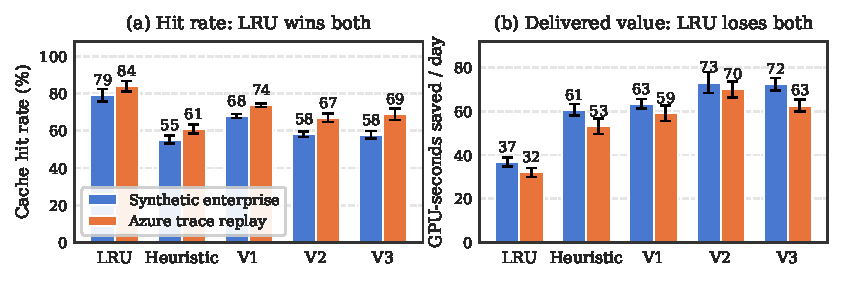
\includegraphics[width=1.0\textwidth]{figures/figure1_reversal.pdf}
  \caption{The same runs, two metrics: LRU wins hit rate on both workloads and delivers the least value on both. 10 paired seeds (synthetic) or ten 6-hour windows (Azure), 95\% t-CIs, 500\,MB.}
  \label{fig:reversal}
\end{figure}

LRU wins the metric we set out to beat, taking the highest hit rate on every constrained workload: 79.1\% [75.9, 82.4] on enterprise against Logistic~V1's 67.9\% [66.8, 69.0], and 96.0\% against 83.9\% on power user.

That verdict is narrower than it sounds. On enterprise traffic (Figure~\ref{fig:reversal}) LRU simultaneously delivers the least value of any policy: V2 saves $1.99\times$ as much GPU time ($+36.4$ GPU-s/day $[+30.4, +42.4]$), V3 $1.97\times$, V1 $1.73\times$, and even the untrained heuristic $1.65\times$, every delta significant. Both replicate on real traffic, and the second strengthens: on the Azure replay LRU again wins hit rate (83.9\%, by 16.9 points over V2) and again delivers the least value, V2 saving $2.18\times$. The inversion is \emph{larger} on real traffic because real sizes are more skewed, so more mass falls below $N^{*}$ (\S\ref{sec:mech}).

\section{Mechanism: A Threshold and a Superlinearity}
\label{sec:mech}

Restoring a persisted cache moves $O(N)$ bytes, while recomputing its prefill costs $O(N)$ weight FLOPs plus $O(N^2)$ attention:
\begin{equation}
  t_{\text{restore}}(N) = \ell_{\text{tier}} + \frac{2 L H_{kv} d b N}{B_{\text{tier}}},
  \qquad
  t_{\text{prefill}}(N) = \frac{2 P N + 4 L H_{q} d N^{2}}{F \eta},
  \label{eq:breakeven}
\end{equation}
for $L$ layers, $H_{kv}$ KV heads (GQA shrinks the cache, not the scores, so query heads $H_q$ appear in prefill), head dimension $d$, $b$ bytes/element, tier latency $\ell$, bandwidth $B$, $P$ parameters, peak $F$ FLOP/s, and utilization $\eta$. Restore is linear and prefill superlinear, so they cross at a break-even length $N^{*}$, set by KV bytes per token over prefill FLOPs per token. That ratio spans four orders of magnitude: on an A100 at $\eta{=}0.45$, $N^{*}$ is 1{,}561 tokens from NVMe (10\,ms, 2\,GB/s) and 25{,}901 from object storage (100\,ms, 500\,MB/s) for TinyLlama-1.1B; 43{,}559 and 254{,}203 for Llama-2-7B; and 12 and 289 for Llama-2-70B, whose GQA shrinks bytes moved while parameters inflate FLOPs avoided. The 7B figure is not a slip: a 512\,KB/token MHA cache is so large against its prefill FLOPs that NVMe offload never repays at realistic contexts. That is why systems shipping KV state compress it~\cite{liu2024cachegen} or use DRAM and RDMA, not a 2\,GB/s disk~\cite{qin2025mooncake}. Our $\eta{=}0.45$ is generous to prefill; higher MFU pushes $N^{*}$ out, not in. The threshold is objective-agnostic too: the same inequality governs time-to-first-token.

Hit rate expresses neither effect. Under TinyLlama economics every cold-tier hit in our token range is worth exactly zero, and LRU, blind to size and tier alike, earns 778 of its 1{,}206 enterprise hits there; above $N^{*}$, meanwhile, savings grow superlinearly, so one 8k-token session can outweigh a dozen 2k-token ones.

% [tb] rather than [t]: at this length the table would otherwise take the top of
% page 4 and push the conclusion onto page 5, past the 4-page body limit.
\begin{table}[b]
\centering
\caption{Two controls decomposing the effect (enterprise, paired seeds; heuristic omitted, see \S\ref{sec:reverse}). \textbf{Middle}: repricing at Llama-2-70B moves $N^{*}$ to 12 tokens, switching the threshold off, and the best margin over LRU falls from $1.99\times$ to $1.08\times$. \textbf{Right}: deleting the cold tier at fixed 500\,MB leaves $1.15\times$.}
\label{tab:controls}
\small
\begin{tabular}{@{}lrrrrrr@{}}
\toprule
 & \multicolumn{2}{c}{TinyLlama, 3-tier} & \multicolumn{2}{c}{Llama-2-70B, 3-tier} & \multicolumn{2}{c}{TinyLlama, 2-tier} \\
\cmidrule(lr){2-3}\cmidrule(lr){4-5}\cmidrule(lr){6-7}
Policy & Hit\% & GPU-s/d & Hit\% & GPU-s/d & Hit\% & GPU-s/d \\
\midrule
LRU           & \textbf{79.1} & 36.8          & \textbf{79.1} & 8{,}173          & \textbf{79.4} & 131.0 \\

Logistic V1   & 67.9 & 63.5                   & 67.9 & \textbf{8{,}806}          & 68.0 & \textbf{150.7} \\
ValDensity V2 & 58.2 & \textbf{73.2}          & 67.1 & 8{,}722                   & 58.5 & 147.4 \\
SpaceTime V3  & 57.8 & 72.4                   & 63.2 & 8{,}783                   & 58.1 & 150.0 \\
\bottomrule
\end{tabular}
\end{table}

Table~\ref{tab:controls} separates them two ways. Repricing at Llama-2-70B, where every hit clears break-even, collapses the enterprise gap to $1.07$--$1.08\times$ and hands power-user traffic back to LRU; the threshold thus accounts for roughly $1.85\times$ and the magnitude effect for the residual ${\sim}1.08\times$. Deleting the cold tier instead, at fixed architecture and 500\,MB, estimates that residual independently at $1.13$--$1.15\times$: V1 and V3 each deliver $1.15\times$ more than LRU while conceding 11 hit-rate points. Two manipulations agreeing within two points isolate the same residual superlinearity. Admission control, by contrast, never helps: V2+AC concedes $4.8$ GPU-s/day to plain V2 on enterprise $[-5.3, -4.3]$ and $6.1$ on the Azure replay $[-6.7, -5.4]$, because under sustained load the cache runs near-full and refusing entries at the door only costs cardinality (App.~\ref{app:ac}).

The same table carries this paper's largest effect, and it is not a policy effect. \emph{Deleting the cold tier raises LRU from 36.8 to 131.0 GPU-s/day, a factor of $3.6$, at identical total capacity}; two-tier LRU beats the best three-tier policy we built by $1.8\times$. The same bytes provisioned differently beat the same bytes managed better, so the $1.99\times$ carries a condition: it holds for a deployment our own model advises against building, and the portable claim is the $1.15\times$ surviving correct provisioning, found only by pricing hits rather than counting them.

\textbf{Ground truth: identical perfect hit rates, different value.}
\label{sec:oracle}
Perhaps the learned policies lose because their predictor is weak (AUC 0.70), not because the objective is wrong. We replay the same traces with \emph{oracle} policies reading the actual future, legitimate because replay is open-loop: \emph{Bélády}~\cite{belady1966replacement}, plus oracle V1 and V3 on ground-truth returns. All three cache perfectly at 100.0\%, so every miss in \S\ref{sec:reverse} is a prediction failure, not a capacity necessity, and LRU trails them $5.70\times$ in value against 20.9 hit-rate points.

That setup yields the cleanest evidence here: every other source of difference is gone. Hit rate cannot distinguish Bélády from Oracle-V3: both read 100.0\%, a paired difference of exactly zero on every seed. Their value differs significantly nonetheless, by $+2.9$ GPU-s/day $[+2.0, +3.8]$ on enterprise, because once nothing need ever be dropped the only decision left is \emph{which tier} holds each entry. The effect is small ($1.4\%$) but real, and hit rate reports it as exactly zero.

\section{Discussion and Conclusion}
\label{sec:caution}

\textbf{Two bugs, both flattering, both ours.} We corrected our own evaluation twice, in opposite directions: a wall-clock replay bug flattered the learned policy, an architecture-free cost model flattered LRU (App.~\ref{app:bugs}). The asymmetry is structural. A policy consuming only access order is insensitive to broken time, features, \emph{and} value models alike; every richer policy is exposed to all three. Harness bugs therefore flatter whichever side depends on the broken component rather than perturbing rankings at random, so LRU comparisons controlling neither replay semantics nor cost-model fidelity deserve re-examination \emph{both} ways.

\textbf{A decision rule, in order of payoff.} (1)~Compute $N^{*}$ per tier from Eq.~\ref{eq:breakeven}: published geometry and storage constants, no measurement. (2)~Do not build tiers whose $N^{*}$ exceeds the workload's context lengths, the largest lever we measured at $3.6\times$. (3)~Refuse admission below the surviving tiers' $N^{*}$, the step our data supports least directly, since density-thresholded admission never helped us and its payoff arrives as step (2). (4)~Only then choose a policy, and never tune on hit rate before establishing the regime.

\textbf{Limitations.} Return behavior and value are both modeled rather than observed; Apps.~\ref{app:cost} and~\ref{app:persona} bound each. No policy we built wins \emph{both} metrics anywhere.

\textbf{Conclusion.} Where a workload straddles $N^{*}$, hit rate ranks KV-cache policies backwards: it picks the worst one available and calls it best. Beating that metric does not require beating LRU.

\bibliographystyle{plainnat}
\bibliography{references}

\appendix

\section{Cost-model validation}
\label{app:cost}

Every value figure in this paper is produced by a model, so the model is the thing most
worth attacking. An earlier version of it deserved the attack: it priced prefill with two
hardcoded constants and no model geometry, placing the linear/quadratic crossover near
1{,}300 tokens where real architectures cross between $12$ and $254$k, and predicting
$57{,}747$\,ms for a 598-token TinyLlama prefill that a T4 measures at ${\sim}37$\,ms. The
model used here (Eq.~\ref{eq:breakeven}) is parameterized by published model geometry and
storage constants instead, and we check it two ways.

\emph{Against hardware.} Table~\ref{tab:costval} sweeps context length on Llama-3.2-1B
(16 layers, GQA 8/32, 32\,KB/token) on a T4 and compares predicted prefill against
measured cold TTFT. Predictions track measurement within $1.15$--$1.66\times$ over a
$12\times$ range of context, and the residual is one-sided: measurement is consistently
slower than prediction, implying an achieved MFU near $0.22$ against the $0.30$ assumed.
The functional form is what matters for our argument, and it holds: over that range cold
prefill grows $14.8\times$ while the warm path grows $1.8\times$.

\emph{Against an independent implementation.} The break-even lengths quoted in
\S\ref{sec:mech} are computed by \texttt{benchmarks/breakeven\_analysis.py} from the same
expressions written separately, and agree exactly with the simulator's cost model at all
three architectures and both tiers. This catches transcription errors, not modeling ones.

\begin{table}[h]
\centering
\caption{Predicted versus measured prefill, Llama-3.2-1B on a T4, five trials per length
(medians). The warm path is tier load plus tensor restore plus one forward pass.}
\label{tab:costval}
\small
\begin{tabular}{@{}rrrrrr@{}}
\toprule
Tokens & Measured prefill & Predicted & Ratio & Measured warm & Predicted restore \\
\midrule
512    & 111\,ms   & 67\,ms    & 1.66$\times$ & 101\,ms & 18\,ms \\
1{,}024 & 157\,ms   & 137\,ms   & 1.15$\times$ & 115\,ms & 27\,ms \\
2{,}048 & 340\,ms   & 288\,ms   & 1.18$\times$ & 115\,ms & 44\,ms \\
4{,}096 & 878\,ms   & 632\,ms   & 1.39$\times$ & 146\,ms & 77\,ms \\
6{,}144 & 1{,}645\,ms & 1{,}032\,ms & 1.59$\times$ & 181\,ms & 111\,ms \\
\bottomrule
\end{tabular}
\end{table}

The fixed cost of the measured warm path is the one constant that does \emph{not}
transfer: fitting it gives 94.5\,ms of overhead plus 13.4\,$\mu$s per token, an implied
2.44\,GB/s against the 2.0\,GB/s the model assumes. The bandwidth transfers; the 94.5\,ms
does not, because a Colab ephemeral disk read through \texttt{torch.load} is not an NVMe
read. $N^{*}$ must therefore be computed from the storage path actually deployed.

\section{Admission control}
\label{app:ac}

\emph{Value Density V2+AC} is V2 plus a value-density admission threshold, derived per run
rather than hardcoded. It never helped on any workload we ran (Table~\ref{tab:ac}), and
the reason is visible in the hit rates: it declines entries at the door without freeing
capacity that the eviction policy would not have freed anyway, so it pays cardinality for
nothing. Under sustained arrivals the cache sits at near-full utilization regardless.

\begin{table}[h]
\centering
\caption{Admission control against plain value density, 10 paired replicates each.
Deltas are per-replicate against V2 with 95\% t-CIs.}
\label{tab:ac}
\small
\begin{tabular}{@{}llrrr@{}}
\toprule
Workload & Policy & Hit\% & GPU-s/day & $\Delta$ vs V2 [CI] \\
\midrule
Synthetic enterprise & ValDensity V2 & 58.2 & \textbf{73.2} & --- \\
                     & V2+AC         & 58.2 & 68.4 & $-4.8$\,$[-5.3, -4.3]$ \\
\midrule
Azure replay         & ValDensity V2 & 67.0 & \textbf{70.0} & --- \\
                     & V2+AC         & 66.8 & 63.9 & $-6.1$\,$[-6.7, -5.4]$ \\
\bottomrule
\end{tabular}
\end{table}

This is a result about \emph{density}-thresholded admission, and it should not be read as
evidence against the $N^{*}$-thresholded admission of step (3) in \S\ref{sec:caution},
which is a different rule and which we do not evaluate as a standalone policy. It is also
conditioned on our accounting flooring sub-$N^{*}$ hits at zero: a policy that merely
declines a worthless hit cannot gain under that floor, and would gain under an accounting
that charged the restore.

\section{The two evaluation defects}
\label{app:bugs}

Both defects were ours, both flattered a different side, and neither perturbed rankings at
random. We report them because the pattern is the transferable part.

\emph{Wall-clock replay (flattered the learned policy).} An early harness replayed a
6-hour trace at wall-clock speed and credited hits with unclamped resume-time token
counts. Collapsing simulated time drives session age, idle time, and hour-of-day to
approximately zero, which zeroes exactly the features the predictor was trained on, while
the accounting credited a different quantity than the policies optimized. It showed a
learned policy beating LRU. Fixing it reversed the result, and we reported LRU winning
both metrics for some time afterwards.

\emph{An architecture-free cost model (flattered LRU).} The simulator priced prefill with
two hardcoded constants, no model geometry at all, placing the linear/quadratic crossover
near 1{,}300 tokens where real architectures cross between $12$ and $254$k. This is not a
rescaling, so the usual invariance argument, that a constant factor cannot change rankings, does not apply: the error inflated an 8k-token session's worth relative to a
512-token one by $3$--$4.5\times$, exaggerating precisely the effect the study measures.
Re-pricing from architecture inverted the value comparison, left hit rates untouched, and
retracted a ``static value density collapses'' finding we had previously reported, which
had been a property of the cost model rather than of the objective.

The reason we caught the second at all is that a reader asked why a 598-token prefill was
modeled at 57.7 seconds when the hardware measured 37 milliseconds. No test in our suite
would have caught it, because none existed; App.~\ref{app:cost} is the test that does now.

\section{Persona strength}
\label{app:persona}

Return behavior in our workloads is generated, not observed, and the dispersion $\sigma$
of per-user return propensity bounds how much structure any predictor can recover. We
sweep it, retraining the predictor at each setting so the model is as good as that world
allows, and re-run the enterprise matrix (Table~\ref{tab:persona}).

\begin{table}[h]
\centering
\caption{Persona strength sweep (enterprise, 5 paired seeds, TinyLlama economics).
Value is GPU-seconds saved per day, as a ratio to LRU.}
\label{tab:persona}
\small
\begin{tabular}{@{}rrrrr@{}}
\toprule
$\sigma$ & Predictor AUC & LRU hit\% & V1 $\times$LRU & V3 $\times$LRU \\
\midrule
0.0 & 0.659 & 95.3 & 0.90 & 1.34 \\
0.3 & 0.670 & 89.5 & 1.47 & 1.50 \\
0.6 & 0.700 & 80.3 & 1.66 & 1.91 \\
1.0 & 0.739 & 66.3 & 1.79 & 2.25 \\
\bottomrule
\end{tabular}
\end{table}

The two claims separate cleanly. The \emph{learned} policy's standing depends on $\sigma$,
as it must: at $\sigma{=}0$, where users are behaviorally identical, V1 falls to
$0.90\times$ LRU and the difference is not significant. A classifier whose premise is
per-user prediction should fail when there is no per-user structure, and it does. The
\emph{metric} finding does not depend on $\sigma$: V3 beats LRU on value at every setting,
and the gap is smallest exactly where LRU is strongest, which is the regime least
favorable to our argument and still not favorable enough to overturn it.

\end{document}
